\chapter{系统设计}
\label{chap:design}

\usetikzlibrary{arrows.meta,positioning,calc}

\begin{figure}[htbp]
\centering
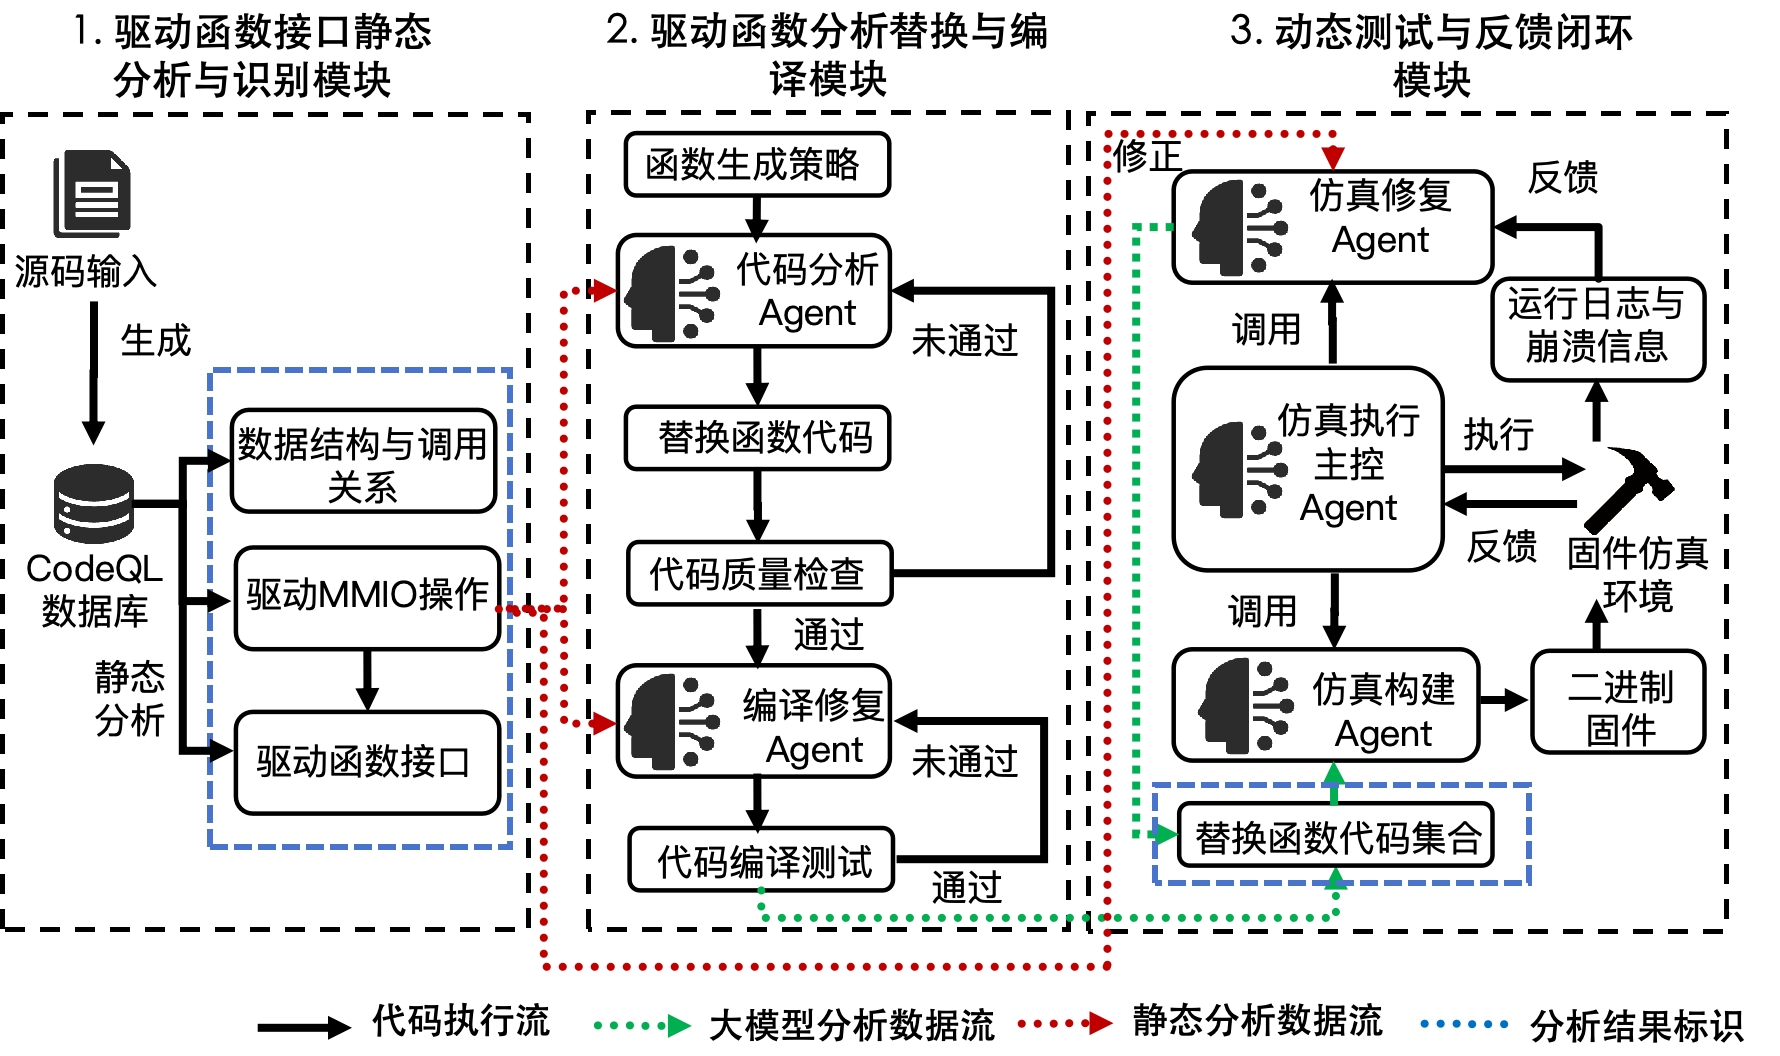
\includegraphics[width=0.95\textwidth]{figures/system_architecture.png}
\caption{系统整体架构图}
\label{fig:arch}
\end{figure}

本研究设计并实现了基于驱动程序替换的固件仿真系统，该系统分为三个模块：（1）驱动函数接口静态分析与识别模块；（2）驱动函数分析、替换与编译模块；（3）动态测试反馈闭环模块。整体方案架构图如图~\ref{fig:arch}所示。

驱动函数接口静态分析与识别模块首先接受固件源码，然后通过 CodeQL 静态分析引擎建立抽象语法树构建的数据库，通过预定义的查询规则从固件源码中提取驱动相关信息，包括驱动函数接口、驱动 MMIO 操作、依赖数据结构与函数间调用关系等信息，并以统一的数据模型对外提供查询接口。

驱动函数分析、替换与编译模块首先接受驱动函数接口静态分析与识别模块输出的驱动函数信息，然后针对各驱动函数进行类型分类并通过合适的函数替换策略生成可替代实现，之后对生成的替换函数代码做质量检查，如果质量检查通过，则将替代实现集成回工程并驱动构建，进一步通过交叉编译验证替换代码是否存在编译错误。如果存在编译错误，则触发编译修复智能体进行修复，修复完成后再次通过交叉编译验证。该模块采用 LangGraph 智能体框架实现复杂的推理和决策流程，确保生成的替换代码既满足语义保持性要求，又能够正常通过交叉编译工具链的验证。

动态测试反馈闭环模块首先接受驱动函数分析、替换与编译模块输出的替换代码，然后在仿真环境中运行固件，采集运行日志、崩溃信息等，并将错误信息结构化，触发闭环修复智能体对嵌入式程序进行重新分析与替换代码修正，修正完成后再次通过闭环构建智能体交叉编译生成可执行的二进制固件程序，再次在仿真环境中运行固件，如此循环，直至替换代码通过仿真测试。通过多智能体协作，该模块构建"生成-测试-反馈-修正"的闭环机制，使固件构建仿真与自修复的全过程实现自动化。

为精确定义系统的输入输出关系，以下给出端到端映射的形式化描述。设固件源码工程为 $P$，固件中的函数集合为 $F$，MMIO 结构体实例集合为 $M$，驱动函数类别集合为 $C$，替换策略集合为 $S$。系统的端到端功能可形式化为以下映射：
\begin{align}
\textit{StaticAnalysis}: P &\to (D, R, G) \label{eq:static} \\
\textit{Classify}: D &\to C \label{eq:classify} \\
\textit{Replace}: D \times C &\to D' \label{eq:replace} \\
\textit{Verify}: D' &\to \{\textit{pass}, \textit{fail}\} \label{eq:verify} \\
\textit{Emulate}: P' &\to (O, E) \label{eq:emulate}
\end{align}
其中，式~\ref{eq:static}~中 $D \subseteq F$ 为识别出的驱动函数集合，$R$ 为 MMIO 访问点集合，$G = (F, E_c)$ 为函数调用图（$E_c$ 为调用边集合）；式~\ref{eq:classify}~将每个驱动函数映射到其语义类别；式~\ref{eq:replace}~对每个驱动函数 $f \in D$ 生成替换实现 $f' \in D'$；式~\ref{eq:verify}~对替换实现进行多层验证；式~\ref{eq:emulate}~中 $P'$ 为替换后的工程，$O$ 为仿真运行输出，$E$ 为运行时错误集合。系统通过迭代执行"替换$\to$验证$\to$仿真$\to$反馈"闭环，直至 $E = \emptyset$ 或达到最大迭代次数。

\section{驱动函数接口静态分析与识别模块设计}

本模块是整个方案的基础支撑层，负责自动、精准地定位固件中与硬件交互的代码，并将其抽象为标准化的"可查询知识库"。模块的核心职责是建立从源码到硬件依赖信息的映射，识别固件中与硬件交互的函数，确定函数访问硬件的方式（如直接寄存器访问、HAL 库调用或间接句柄操作），并分析函数之间的调用依赖关系。

在静态分析引擎的选型上，本模块需要对比源码级方案内部的两种技术路线：基于 LLVM/Clang 的分析和基于 CodeQL 的分析。

基于 LLVM/Clang 的分析方案（如 P2IM~\cite{fengp2020p2im} 采用基于 LLVM IR 的启发式规则识别外设寄存器访问）在实际应用中面临工程兼容性问题。嵌入式固件的构建工具链通常与 ARM GCC 深度绑定：Zephyr RTOS 通过 west 构建系统默认调用 \texttt{arm-none-eabi-gcc} 进行交叉编译，STM32CubeIDE、MCUXpresso 等厂商 IDE 同样基于 ARM GCC 工具链；嵌入式工程中广泛使用的 CMSIS 头文件、芯片厂商提供的设备描述头文件以及 \texttt{\_\_attribute\_\_}、\texttt{\_\_IO}、\texttt{\_\_ASM} 等 ARM GCC 扩展语法，Clang 的兼容性尚不完整。若采用基于 Clang 的源码分析工具，需要将整个构建工具链从 ARM GCC 切换到 Clang，这一过程涉及重新配置构建系统、适配厂商头文件中的编译器扩展语法以及处理链接器脚本差异等问题，迁移成本较高。此外，部分嵌入式工程的构建脚本使用 ARM GCC 特有的编译选项（如 \texttt{-mcpu=cortex-m4}、\texttt{-mfpu=fpv4-sp-d16} 等），Clang 对这些选项的语义解释存在差异，可能导致分析结果与实际编译行为不一致。

CodeQL 采用与编译器无关的数据库构建方式：通过在构建过程中拦截编译器调用来捕获源码信息，而非替代原始编译器执行编译。因此，CodeQL 可以直接在 ARM GCC 工具链的构建流程上工作，无需修改固件工程的编译配置。CodeQL 将源码构建为包含 AST、控制流图和数据流图的综合数据库，支持声明式查询语言和全局污点追踪，能够在不运行固件的情况下跨文件追踪 MMIO 基址常量的传播路径，为后续的智能替换提供基础数据。与运行时方法相比（如 HALucinator~\cite{clements2020halucinator} 通过 QEMU 的内存追踪识别外设访问），CodeQL 无需先实现完整的外设模型即可工作。

模块采用静态分析技术构建包含语法树、控制流图和数据流图的综合数据库，通过设计的查询规则识别 MMIO 结构体实例和字段访问，进而识别涉及硬件访问的驱动函数，为替换模块提供精确的语句定位信息。模块输出的分析结果包含驱动函数列表、MMIO 访问操作、函数调用关系图和数据结构信息，这些结构化的分析结果被存储在统一的数据模型中，为下游模块提供可查询的知识库。

\subsection{MMIO 访问模式识别方法}

MMIO（Memory-Mapped I/O，内存映射 I/O）是一种将硬件外设的寄存器映射到处理器内存地址空间的机制。通过 MMIO，软件可以通过访问内存地址的方式与硬件外设进行交互，而不需要特殊的 I/O 指令。嵌入式厂商通常使用 C 语言结构体来定义 MMIO 寄存器映射，结构体的每个字段对应一个硬件寄存器，字段的偏移量与硬件规范中的寄存器地址偏移保持一致。

MMIO 结构体的典型代码示例如代码~\ref{lst:mmio-struct}所示。

\begin{lstlisting}[style=CStyle,language=C,caption=MMIO 结构体示例,label=lst:mmio-struct]
// STM32 UART寄存器映射示例
typedef struct {
    __IO uint32_t CR1;    // 控制寄存器1
    __IO uint32_t CR2;    // 控制寄存器2
    __IO uint32_t CR3;    // 控制寄存器3
    __IO uint32_t BRR;    // 波特率寄存器
    __IO uint32_t GTPR;   // 保护时间与预分频寄存器
    __IO uint32_t RTOR;   // 接收超时寄存器
    __IO uint32_t RQR;    // 请求寄存器
    __IO uint32_t ISR;    // 中断与状态寄存器
    __IO uint32_t ICR;    // 中断标志清除寄存器
    __IO uint32_t RDR;    // 接收数据寄存器
    __IO uint32_t TDR;    // 发送数据寄存器
} USART_TypeDef;

// 通过强制类型转换创建MMIO实例
#define USART1_BASE    (0x40011000UL)
USART_TypeDef *USART1 = (USART_TypeDef *)USART1_BASE;
\end{lstlisting}

定位 MMIO 结构体实例是识别硬件相关代码的关键步骤。本研究总结出三种典型的 MMIO 实例定位模式，分别如代码~\ref{lst:direct-cast}、代码~\ref{lst:indirect-init}和代码~\ref{lst:pointer-param}所示。

\textbf{模式一：直接地址强转}。这类代码将固定外设基地址强制转换为外设寄存器结构体指针，常见于寄存器定义的头文件中。在代码中呈现为类似 \texttt{\#define USART1 ((USART\_TypeDef *)USART1\_BASE)} 的宏定义，后续代码直接对该指针进行字段访问如 \texttt{USART1->DR}、\texttt{USART1->CR1}。

\begin{lstlisting}[style=CStyle,language=C,caption=直接地址强转模式示例,label=lst:direct-cast]
// 驱动源码示例：直接地址强转模式
#define USART1_BASE 0x40011000UL
#define USART1 ((USART_TypeDef *)USART1_BASE)
#define USART2 ((USART_TypeDef *)USART2_BASE)
#define USART3 ((USART_TypeDef *)USART3_BASE)

void uart_init_direct(void) {
    USART1->CR1 = 0x2000;  // 直接对强转实例进行寄存器访问
    USART1->BRR = 0x0341;
}
\end{lstlisting}

\textbf{模式二：间接初始化}。这类代码通过句柄（handle）、配置表（descriptor/config table）等间接结构，将外设基地址赋值给某个"寄存器块指针成员"，后续通过该成员完成寄存器访问。在 STM32 HAL 生态中，这类成员常命名为 \texttt{Instance}。在代码中呈现为初始化时的赋值语句如 \texttt{huart->Instance = COM\_USART[COM]}，后续寄存器访问呈现为多级解引用如 \texttt{huart->Instance->DR}。在基于配置表的驱动中，也可能呈现为 \texttt{handle.Instance = spi\_config[i].Instance} 这种从配置表复制的形式。

\begin{lstlisting}[style=CStyle,language=C,caption=间接初始化模式示例（HAL句柄和配置表）,label=lst:indirect-init]
// 驱动源码示例：间接初始化模式（HAL句柄）
UART_HandleTypeDef huart;

void BSP_COM_Init(COM_TypeDef COM) {
    huart.Instance = COM_USART[COM];  // 将外设基地址赋值给Instance成员
    HAL_UART_Init(&huart);
    // 后续访问呈现为多级解引用
    huart.Instance->DR = data;
}

// 驱动源码示例：间接初始化模式（配置表）
typedef struct {
    USART_TypeDef *Instance;
    uint32_t BaudRate;
} SPI_Config;

SPI_Config spi_config[] = {
    {SPI1, 115200},
    {SPI2, 9600}
};

void rt_hw_spi_bus_init(void) {
    for (int i = 0; i < sizeof(spi_config)/sizeof(spi_config[0]); i++) {
        spi_bus_obj[i].handle.Instance = spi_config[i].Instance;
        // 通过配置表中的Instance赋值
    }
}
\end{lstlisting}

\textbf{模式三：常量指针参数}。这类代码通过函数参数接收 MMIO 结构体指针（寄存器块基址），常见于底层驱动或通用外设操作函数。在代码中呈现为函数定义的形参类型是某个寄存器结构体指针，函数体内部通过该参数访问寄存器字段，如 \texttt{void mmio\_uart\_init(USART\_TypeDef *uart) \{ uart->CR1 = 0x2000; \}}。调用者可以将模式一或模式二中的 MMIO 实例作为实参传入，如直接调用 \texttt{mmio\_uart\_init(USART1)} 或传入句柄成员 \texttt{mmio\_uart\_init(huart.Instance)}。

\begin{lstlisting}[style=CStyle,language=C,caption=常量指针参数模式示例,label=lst:pointer-param]
// 驱动源码示例：常量指针参数模式
void mmio_uart_init_pointer(USART_TypeDef *uart) {
    // 通过指针访问MMIO寄存器
    uart->CR1 = 0x2000;
    uart->BRR = 0x0341;
}

// 调用示例
void main(void) {
    // 直接传模式一的强转实例
    mmio_uart_init_pointer(USART1);

    // 传模式二的句柄成员
    mmio_uart_init_pointer(huart.Instance);

    return 0;
}
\end{lstlisting}

三种定位模式的对比如表~\ref{tab:mmio-patterns}所示。

设 $T$ 为 MMIO 寄存器结构体类型集合，$A$ 为外设基址常量集合，$H$ 为句柄结构体类型集合，$F$ 为函数集合，则三种定位模式可形式化定义为：

\textbf{模式一（直接地址强转）}：存在常量 $a \in A$ 和类型 $t \in T$，使得 $a$ 被显式转换为 $t^*$ 类型，即存在表达式 $\texttt{cast}(a) \to t^*$。后续通过该指针的字段访问构成 MMIO 操作：
$$\textit{DirectCast} = \{(a, t) \mid a \in A, t \in T, \exists\, \texttt{cast}(a): a \to t^*\}$$

\textbf{模式二（间接初始化）}：存在句柄 $h$（类型为 $\tau \in H$），其成员 $h.\textit{inst}$ 被赋值为 MMIO 实例的指针，后续通过 $h.\textit{inst} \to \textit{field}$ 进行字段访问：
$$\textit{IndirectInit} = \{(h, t) \mid h.\textit{inst} = \textit{ptr}, \textit{ptr} \to t^*, t \in T\}$$

\textbf{模式三（常量指针参数）}：存在函数 $f \in F$，其参数列表中包含类型为 $t^*$（$t \in T$）的形式参数，调用点传入 MMIO 实例指针作为实参：
$$\textit{PtrParam} = \{(f, t, i) \mid f.\textit{param}_i: t^*, t \in T\}$$

三种模式共同构成 MMIO 实例的完整识别规则集合 $\textit{MMIOInst} = \textit{DirectCast} \cup \textit{IndirectInit} \cup \textit{PtrParam}$。与已有方法不同，P2IM~\cite{fengp2020p2im} 通过运行时 fuzzing 探测外设行为，HALucinator~\cite{clements2020halucinator} 通过 QEMU 内存追踪识别外设访问，本研究从源码层面对 MMIO 访问模式进行了系统性的分类和形式化描述，为驱动函数的精确识别提供了可复用的查询规则。

\begin{table}[htbp]
\centering
\caption{MMIO 结构体实例定位模式对比}
\label{tab:mmio-patterns}
\footnotesize
\begin{tabular}{lp{5cm}l}
\toprule
\textbf{模式} & \textbf{描述} & \textbf{代码呈现} \\
\midrule
直接地址强转 & 将固定地址强制转换为外设结构体指针 & 整数常量$\to$结构体指针类型转换 \\
间接初始化 & 通过配置表将外设基地址赋值给句柄 & 结构体成员赋值为外设宏 \\
常量指针参数 & 函数以常量指针形式接收外设基址 & 参数类型为 MMIO 结构体指针 \\
\bottomrule
\end{tabular}
\end{table}

\subsubsection{查询规则设计原则}

为在 CodeQL 数据库中可靠地识别上述三种 MMIO 定位模式，本研究设计了相应的查询规则体系。查询规则的设计遵循以下原则：

\textbf{（1）结构体特征识别}。首先识别 MMIO 寄存器结构体，判定依据包括：结构体名称包含 \texttt{TypeDef}、\texttt{\_TypeDef}、\texttt{\_Registers} 等典型后缀；结构体字段类型以 \texttt{\_\_IO}（volatile 修饰）为主；字段偏移量与芯片参考手册中的寄存器地址偏移一致。查询规则通过匹配这些特征从数据库中提取候选 MMIO 结构体，过滤掉普通数据结构体。

\textbf{（2）基址常量识别}。MMIO 实例的基址通常以宏或枚举常量的形式定义，其数值范围为典型外设地址区间（如 STM32F4 的 APB1/APB2 总线地址 0x40000000--0x50000000）。查询规则通过识别数值落在已知外设地址区间内的常量表达式，过滤掉地址空间无关的普通整数常量，降低误报率。

\textbf{（3）类型转换链追踪}。对于模式一（直接地址强转），查询规则追踪从基址常量到结构体指针类型的显式转换表达式（C 语言中的 \texttt{(Type *)cast} 形式），并进一步追踪通过该指针的解引用和字段访问。对于模式二（间接初始化），查询规则通过数据流追踪识别从 MMIO 实例到句柄成员的赋值传播路径，再追踪句柄成员的字段访问。对于模式三（常量指针参数），查询规则匹配函数参数类型为 MMIO 结构体指针的函数定义，并追踪调用点传入的实际参数来源。

\textbf{（4）污点传播与边界控制}。为防止追踪范围过度扩散，查询规则设置传播边界条件：仅追踪通过指针解引用（\texttt{->} 操作符）和结构体字段访问的路径，不追踪算术运算后的指针偏移；传播深度限制在函数调用图的三层以内，避免跨模块追踪引入无关噪声。对于跨文件和跨编译单元的 MMIO 访问，通过 CodeQL 的全局数据流分析能力实现跨文件追踪。

上述查询规则的设计确保了 MMIO 识别的准确性和可扩展性：结构体特征识别和基址常量识别提供了高精度的起点，类型转换链追踪覆盖了三种定位模式的代码呈现形式，污点传播边界控制则在保证召回率的同时限制了误报范围。当需要支持新的 MCU 平台时，仅需更新基址常量的地址区间和结构体特征的后缀规则即可适配，无需修改核心查询逻辑。

\subsection{驱动函数定位准则}

静态分析模块的核心任务是识别固件中的驱动函数。本研究采用简单直接的定位准则：\textbf{凡是包含 MMIO 访问的函数，均定义为驱动函数}。这一定位准则的合理性在于：MMIO 访问是固件与硬件交互的最底层方式，包含寄存器读写的函数必然与硬件强相关，这类函数在仿真环境中无法直接执行，需要进行替换处理；而不包含 MMIO 访问的函数通常是纯软件逻辑，如数据处理、协议解析、状态管理等，在仿真环境中可以直接运行，无需替换。

设 $F$ 为固件中的函数集合，$M$ 为 MMIO 结构体实例集合，$A(f, m)$ 为谓词"函数 $f$ 访问 MMIO 实例 $m$ 的字段"，则驱动函数集合 $D$ 定义为：
$$D = \{f \in F \mid \exists m \in M: A(f, m)\}$$

驱动函数识别的流程如下：首先通过三种定位模式识别代码中的所有 MMIO 结构体实例；然后对每个 MMIO 结构体实例，追踪其字段访问表达式，记录访问的字段名、访问类型（读/写）、所在语句和所在函数；接着对所有包含 MMIO 字段访问的函数进行汇总，形成驱动函数列表；最后分析驱动函数之间的调用关系，构建函数调用图。

\subsection{数据流追踪方法}

系统以"MMIO 字段访问"为源点，以"函数参数、局部变量、返回值"为汇点，构建数据流配置并追踪路径。追踪目的包括：

1. 确定哪些函数参数最终影响了 MMIO 访问；
2. 识别需要保留的业务逻辑与需要替换的硬件操作；
3. 为替换模块提供精确的语句定位信息。

\subsubsection{追踪配置设计}

数据流追踪基于 CodeQL 提供的污点分析框架实现。系统配置了两类追踪路径：

\textbf{正向追踪}：从 MMIO 基址常量出发，沿赋值语句、函数参数传递、结构体字段赋值等路径追踪 MMIO 实例的传播，识别所有通过该实例进行字段访问的代码位置。正向追踪的源点为识别出的 MMIO 基址常量表达式，汇点为结构体字段访问表达式（即 \texttt{expr->field} 形式的访问）。

\textbf{反向追踪}：从 MMIO 字段访问表达式出发，反向追踪数据来源，确定访问的值是否来源于函数参数或外部输入。反向追踪用于区分"配置型访问"（值由软件写入寄存器，如初始化阶段设置波特率）和"状态型访问"（值从寄存器读出，如轮询等待标志位），前者通常可安全替换，后者需要通过仿真注入接口模拟硬件状态。

\subsubsection{追踪复杂度分析}

设固件中函数数量为 $n$，平均函数调用深度为 $d$，平均每个函数的 MMIO 访问点数量为 $k$。数据流追踪的时间复杂度取决于 CodeQL 污点分析引擎的实现，其理论复杂度为 $O(n \cdot d \cdot k)$：$n$ 为候选源点函数的数量，$d$ 为追踪的最大传播深度（受边界条件约束），$k$ 为每个函数中需要检查的汇点数量。在本研究的测试固件中，$n$ 的取值范围为 10--130，$d$ 通常不超过 5，$k$ 的平均值约为 3，因此单次追踪的计算开销在可接受范围内。空间复杂度为 $O(n \cdot d)$，主要用于存储追踪路径的中间结果。

需要指出的是，CodeQL 的污点分析基于静态近似，可能存在以下局限：一是无法处理通过函数指针或虚函数表进行的间接调用，这类间接调用在嵌入式固件中相对少见；二是对运行时才能确定的数组索引和条件分支采用保守估计，可能引入少量无关追踪路径。在实际应用中，上述局限对驱动函数识别的召回率影响有限，因为嵌入式驱动代码的函数调用关系通常较为明确，间接调用的使用场景较少。

\subsection{统一数据模型设计}

系统定义了统一的数据模型来表示分析结果，包括 \texttt{FunctionInfo}（函数基本信息）、\texttt{MMIOAccess}（MMIO 访问点）等结构，为上层模块提供标准化查询接口。数据模型采用 Python 数据类（dataclass）定义，支持序列化和反序列化。

数据模型包括函数信息模型（包含函数名、文件路径、行号、签名、返回类型、参数列表、分类、源码、调用关系等信息）、MMIO 访问点模型（包含结构体类型、字段名、访问类型、行号、所在函数、上下文代码等）和项目分析结果模型（包含项目路径、CodeQL 数据库路径、所有函数、MMIO 访问点、函数调用图、驱动函数列表、分析时间戳等）。这些数据模型通过 JSON 序列化存储在缓存层，供后续模块查询和使用。

\section{驱动函数分析、替换与编译模块设计}

驱动函数分析、替换与编译模块负责语义理解和代码生成，采用大语言模型驱动的智能体架构，实现从函数分类、代码生成、质量验证到编译集成的完整自动化流程。该模块采用"语义分析$\to$代码生成$\to$质量验证$\to$编译集成$\to$错误修复"的迭代优化模式，通过多轮迭代逐步提升替换质量，直至生成能够在仿真环境中正常运行的替换代码。

在智能体框架的选型上，本模块选择 LangGraph 作为编排框架。驱动函数替换涉及多轮推理决策（函数分类、策略选择、代码生成、质量验证），且各步骤之间存在复杂的条件依赖和迭代关系。LangGraph 基于图式状态机模型，天然支持条件分支和循环结构，能够精确表达"分类→生成→验证→修复"的迭代工作流；同时支持工具调用（Tool Calling）机制，可以将静态分析查询、编译构建等外部能力封装为图节点，实现智能体与工程环境的深度集成。相比纯对话式框架，LangGraph 对执行流程的控制粒度更细，能够精确控制每步的输入输出和状态传递，这对于需要严格保证函数签名一致性和编译正确性的驱动替换场景尤为必要。

\subsection{分析替换与编译智能体工作流设计}

工作流以\textbf{单个驱动函数}为粒度调度：每轮从静态分析模块或任务队列中取定一条驱动函数记录（含签名、源码片段、MMIO 访问上下文等），在图式状态机中顺序执行，直至该函数被判定为无需替换并结束，或替换实现通过校验与编译并被采纳。为便于叙述与实现解耦，整条流水线在逻辑上划分为\textbf{驱动函数分析与替换代码生成}、\textbf{替换代码修正与编译集成}两个子模块；前者由\textbf{分析智能体}主导完成上下文拉取、分类与候选替换生成，后者由\textbf{编译修复智能体}在工程侧完成定义校验、构建与失败修复。为避免混淆，下文将模块二中的编译修复智能体称为"编译修复智能体"，将模块三中负责运行时错误后重新构建的智能体称为"闭环构建智能体"，两者职责不同：前者处理替换代码首次集成时的编译错误（如语法错误、类型不匹配），后者处理动态反馈闭环中经仿真验证发现运行时错误后的重新构建。

\begin{figure}[htbp]
    \centering
    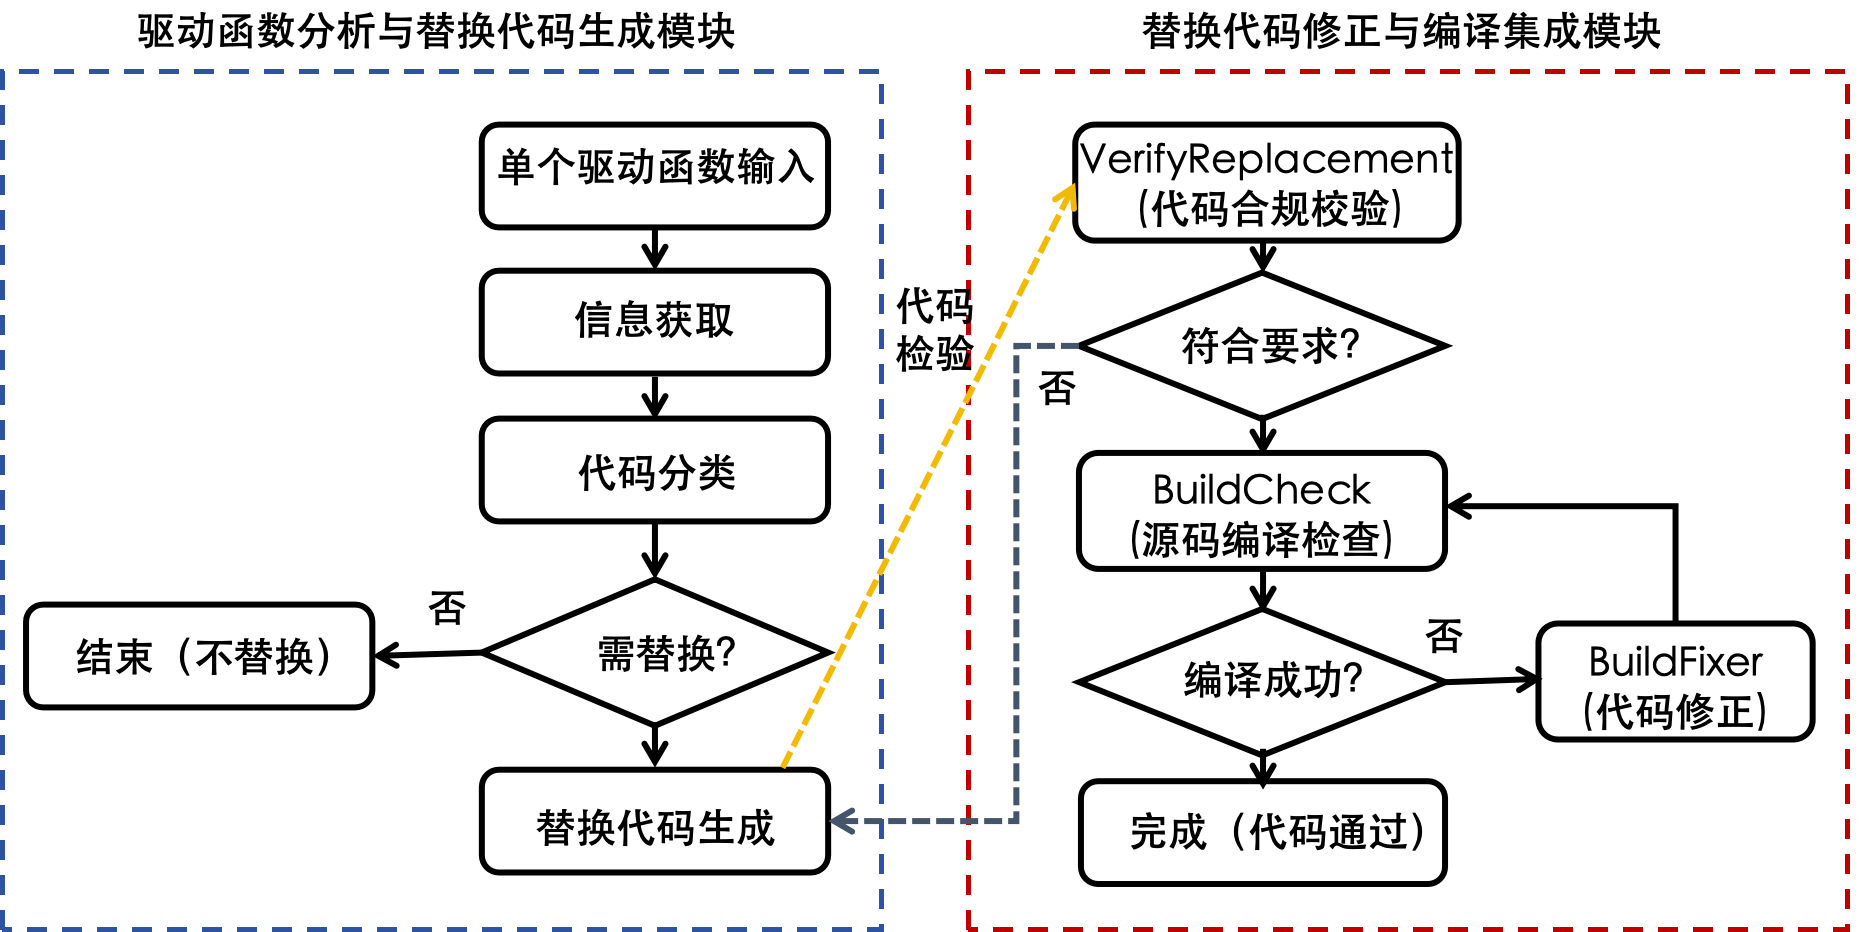
\includegraphics[width=\textwidth]{figures/驱动函数分析替换与编译.png}
    \caption{驱动函数分析替换编译模块示意图}
    \label{fig:analyzer-workflow}
\end{figure}

\subsubsection{驱动函数分析与替换代码生成模块设计}
\label{sec:analyzer-workflow}

该子模块由\textbf{分析智能体}驱动，在 LangGraph 状态机中通过"工具调用—推理—写回"的循环完成单函数处理。执行顺序固定为：\textbf{信息获取} $\to$ \textbf{代码分类} $\to$（仅在分类结果认定该函数需要替换时）\textbf{替换代码生成}。

\textbf{信息获取}阶段通过工具调用获取该驱动函数在工程中的完整上下文，包括完整实现或相关片段、函数签名与参数类型、调用关系与 MMIO 仿真侧提示等（如 GetFunctionInfo、GetFunctionCallStack、GetMMIOFunctionEmulateInfo）。\textbf{代码分类}阶段综合源码与静态分析结果，由大语言模型判定函数语义类别及是否属于必须替换的硬件相关行为；分类所依据的类别体系及提示构造方式见第~\ref{sec:driver-replacement-strategy}~节。\textbf{替换代码生成}仅在"需要替换"分支上触发：模型在既定类别上选择替换策略并产出与签名一致的候选实现，具体策略（如 Skip、Strip、Redirect、Event 等）的选择规则与生成约束同样在第~\ref{sec:driver-replacement-strategy}~节展开，本节只给出子模块内的先后次序与数据交接关系。

\subsubsection{替换代码修正与编译集成模块设计}
\label{sec:builder-workflow}

该子模块在工程目录中对上一子模块输出的\textbf{候选替换代码}做\textbf{二阶段检验与修复}，目标是在真实构建环境下得到可链接、可编译的替换定义。

\textbf{第一阶段（代码合规校验）}调用 VerifyReplacement，依据预置规则与接口契约检查候选替换是否满足替换定义（例如签名一致、禁止引入不兼容的存储类或明显违背仿真假设的写法等），过滤与定义明显不符的实现；未通过时可将反馈交回分析智能体侧重新生成或局部修订（图~\ref{fig:analyzer-workflow}中以虚线表示返回替换生成环节）。

\textbf{第二阶段（语法编译检查）}在通过定义校验后，将替换写入目标源文件（如 ReplaceFuncs，并保留回滚所需的原定义快照），再调用工程构建脚本执行完整编译链接（如 BuildProject）。若\textbf{编译失败}，则进入编译修复智能体路径：由编译修复智能体解析编译器诊断信息，结合 GetFunctionInfo、GetMMIOFunctionInfo 等工具定位首个关键错误，通过 UpdateFunctionReplacement 或 FixFunctionBuildErrors 等动作修订替换代码，并再次触发构建，形成"编译 $\to$ 错误解析 $\to$ 修复 $\to$ 重新编译"的闭环，直至编译成功或达到步数上限，从而保证最终被采纳的替换函数能够通过工程编译。

编译错误的典型成因包括函数未声明、类型不匹配、缺少头文件、链接错误，以及替换代码引用了目标芯片 HAL 中不存在的结构体成员或与头文件声明不一致等。例如，STM32F401 的 TIM\_HandleTypeDef 无 ErrorCode 成员、RCC\_PLLInitTypeDef 无 PLLR 成员时，若替换体仍访问这些成员会导致编译失败；将非静态函数误写为 static 亦会破坏链接一致性。编译修复智能体针对不同诊断采取补声明、改类型与转换、补 \texttt{\#include}、删改非法成员访问、核对依赖等策略。提示词上约束智能体在构建失败时优先根据 stderr 锁定\textbf{第一个错误}所涉函数再查上下文，避免对多函数无序轮询而浪费工具调用次数，从而兼顾修复质量与效率。

\subsection{驱动函数替换策略设计}
\label{sec:driver-replacement-strategy}

为实现语义保持的驱动函数替换，本研究在替换前先对驱动函数进行语义分类，并基于分类结果选择对应替换策略，避免硬件依赖被误删或替换不足导致仿真异常。

\subsubsection{函数分类策略设计}

驱动函数替换的核心挑战在于不同类型的驱动函数与硬件交互的方式和语义要求存在显著差异。采用无差别的统一替换策略无法准确处理各类函数的特殊性，容易导致仿真异常或语义丢失。因此，系统在替换前先对驱动函数进行语义分类，根据函数类别选择最合适的替换策略，从而确保替换后代码的正确性和仿真环境的稳定性。

系统基于大语言模型实现驱动函数的自动分类。LLM 通过读取函数源码、识别 MMIO 访问模式、判断函数主要用途等步骤，将函数分类到预定义的类别。分类策略基于对嵌入式驱动函数硬件交互模式的分析，将函数划分为以下类别，如表~\ref{tab:function-categories}所示。

设驱动函数集合 $D$ 上的分类映射定义为：
$$\textit{classify}: D \to C = \{\textit{INIT}, \textit{RECV}, \textit{LOOP}, \textit{IRQ}, \textit{RETURNOK}, \textit{SKIP}, \textit{CORE}, \textit{NODRIVER}\}$$

对于需要替换的函数子集 $D_r = \{f \in D \mid \textit{classify}(f) \in C \setminus \{\textit{CORE}, \textit{NODRIVER}\}\}$，系统进一步为其分配替换策略。替换策略映射定义为：
$$\textit{strategy}: D_r \to S = \{\textit{Skip}, \textit{Redirect}, \textit{Event}, \textit{Steering}, \textit{ReturnOK}\}$$

该分类体系旨在解决已有方法中替换策略与函数语义不匹配的问题。HALucinator~\cite{clements2020halucinator} 采用统一的 HAL profile 拦截策略，P2IM~\cite{fengp2020p2im} 通过随机 fuzzing 生成外设响应，均未对驱动函数的语义类别进行系统性区分。当替换策略与函数语义不匹配时，容易出现仿真异常——例如 LOOP 类函数未移除轮询逻辑引发死循环、RECV 类函数未注入模拟数据导致上层协议栈读取到无效值。本研究通过"先分类后替换"的范式，使每类函数获得与其语义特征相匹配的替换策略，从设计层面降低了替换导致的语义错误风险。

\subsubsection{分类判定规则}

为提高分类的准确性和一致性，系统为每类函数定义了明确的判定规则，LLM 在分类时需综合以下特征进行判定：

\textbf{（1）INIT 类判定规则}。满足以下条件之一的函数归类为 INIT：函数名包含 \texttt{Init}、\texttt{Config}、\texttt{Setup}、\texttt{MspInit} 等关键词；函数体内包含对多个 MMIO 寄存器的顺序写操作且无读-改-写循环；函数调用位置位于系统启动阶段或外设初始化流程中（通过调用图判断）。INIT 类函数的特征是对硬件进行一次性配置，执行后不依赖返回的硬件状态。

\textbf{（2）RECV 类判定规则}。满足以下条件之一的函数归类为 RECV：函数名包含 \texttt{Receive}、\texttt{Read}、\texttt{Get}、\texttt{Input} 等关键词；函数体内包含从 MMIO 数据寄存器（如 \texttt{RDR}、\texttt{DR}、\texttt{RXDATA}）的读操作；函数参数中包含目标缓冲区指针和长度参数。RECV 类函数的核心语义是从硬件获取数据并传递给上层软件，替换时需要通过仿真注入接口提供模拟数据。

\textbf{（3）LOOP 类判定规则}。满足以下条件之一的函数归类为 LOOP：函数名包含 \texttt{Wait}、\texttt{Poll}、\texttt{Loop} 等关键词；函数体内包含以 MMIO 状态寄存器（如 \texttt{ISR}、\texttt{SR}）的某一位为条件的循环结构（\texttt{while(flag == RESET)} 形式）；循环体内部无实质性的数据处理逻辑，仅为等待硬件状态变化。LOOP 类函数在仿真环境中会造成死循环，必须通过 Skip 策略移除等待逻辑。

\textbf{（4）IRQ 类判定规则}。满足以下条件之一的函数归类为 IRQ：函数名包含 \texttt{IRQHandler}、\texttt{Callback}、\texttt{Handler} 等关键词；函数被注册为中断服务例程（通过中断向量表或 \texttt{HAL\_RegisterCallback} 等方式）；函数体内包含对 MMIO 中断状态寄存器的读操作和清标志操作。IRQ 类函数的触发依赖硬件中断信号，在仿真环境中需要通过 Event 策略将其改造为可由仿真器主动触发的事件处理函数。

\textbf{（5）RETURNOK 类判定规则}。满足以下条件之一的函数归类为 RETURNOK：函数仅包含单个或少量简单的 MMIO 读操作且不使用读出值；函数的返回类型为状态枚举（如 \texttt{HAL\_StatusTypeDef}）且所有执行路径均返回成功状态；函数的语义等价于"检查硬件状态并返回成功"。RETURNOK 类函数在仿真环境中无需执行具体操作，直接返回成功状态值即可。

\textbf{（6）SKIP 类判定规则}。满足以下条件之一的函数归类为 SKIP：函数返回类型为 \texttt{void} 且函数体内的 MMIO 操作对固件状态机无影响；函数名包含 \texttt{DeInit}、\texttt{MspDeInit}、\texttt{Flush} 等资源释放类关键词；函数的功能仅为清理硬件状态或重置外设寄存器。SKIP 类函数在仿真环境中可以直接跳过执行。

\textbf{（7）CORE 类判定规则}。满足以下条件之一的函数归类为 CORE：函数属于操作系统内核代码（如 \texttt{rt\_thread\_init}、\texttt{SysTick\_Handler}）；函数的实现由仿真器直接提供，不经过替换流程。CORE 类函数由系统预配置，不参与 LLM 分类。

\textbf{（8）NODRIVER 类判定规则}。函数虽位于驱动模块中，但满足以下全部条件：函数体内不包含直接的 MMIO 寄存器访问；函数的功能为纯软件逻辑（如参数校验、错误码转换、辅助计算）；函数的执行不依赖任何硬件状态。NODRIVER 类函数在仿真环境中可直接运行，无需替换。

上述判定规则以结构化的形式嵌入 LLM 的分类提示模板中，指导模型从函数名、MMIO 访问模式、控制流结构和调用上下文四个维度综合判断，从而提高分类的一致性。当函数特征同时满足多个类别的判定条件时，LLM 根据函数的主要语义选择最合适的类别，优先级规则为：CORE > IRQ > RECV > LOOP > INIT > RETURNOK > SKIP > NODRIVER。

\begin{table}[htbp]
\centering
\caption{驱动函数分类体系}
\label{tab:function-categories}
\footnotesize
\setlength{\tabcolsep}{4pt}
\begin{tabular}{@{}llp{6.6cm}@{}}
\toprule
\textbf{缩写} & \textbf{描述} & \textbf{典型函数} \\
\midrule
INIT & 外设初始化，影响固件状态机 & \texttt{HAL\_UART\_Init}, \texttt{BOARD\_BootClockRUN} \\
RECV & 从硬件/DMA 读取数据 & \texttt{HAL\_UART\_Receive}, \texttt{ENET\_GetRxFrame} \\
LOOP & 轮询等待硬件状态 & \texttt{HAL\_UART\_WaitOnFlag}, \texttt{FLASH\_WaitForLastOperation} \\
IRQ & 中断处理/回调函数 & \texttt{HAL\_UART\_IRQHandler}, \texttt{ENET\_TransmitIRQHandler} \\
RETURNOK & 纯硬件操作，返回状态值 & \texttt{HAL\_GPIO\_DeInit}, \texttt{HAL\_I2C\_IsDeviceReady} \\
SKIP & 纯硬件操作，无返回值 & \texttt{HAL\_ADC\_MspInit}, \texttt{FLASH\_FlushCaches} \\
\midrule
CORE & 系统区操作，OS 核心函数 & \texttt{SysTick\_Handler}, \texttt{rt\_thread\_init} \\
NODRIVER & 存在的驱动操作对固件状态机无影响 & \texttt{main}, \texttt{GPIO\_GetInstance} \\
\bottomrule
\end{tabular}
\end{table}

这八类函数覆盖了嵌入式固件中与硬件交互的各种典型模式。其中，INIT、RECV、LOOP、IRQ、RETURNOK 和 SKIP 六类函数均直接或间接地涉及 MMIO 寄存器访问，需要通过替换消除硬件依赖；CORE 类函数涉及操作系统核心功能（如系统定时器、线程调度），由仿真器直接提供底层支持，无需替换；NODRIVER 类函数虽然存在于驱动模块中，但其操作对固件状态机无影响或属于纯业务逻辑，同样无需替换。该分类体系的设计兼顾了完备性和实用性，确保每类函数都有明确的替换策略或处理方式。

\subsubsection{替换策略体系设计}

本研究总结出五种通用替换策略，每种策略适用于特定的函数类别和使用场景。表~\ref{tab:replace-strategies}展示了各类函数与替换策略的对应关系，策略的选择由 LLM 根据函数的语义特征自动决定。

\begin{table}[htbp]
\centering
\caption{替换策略选择指南}
\label{tab:replace-strategies}
\footnotesize
\setlength{\tabcolsep}{4pt}
\begin{tabular}{@{}llp{5.9cm}@{}}
\toprule
\textbf{函数类别} & \textbf{策略类型} & \textbf{说明} \\
\midrule
INIT & Skip/Steering & 移除硬件寄存器操作，保留结构体初始化，避免仿真环境中的阻塞 \\
RECV & Redirect/Steering & 利用 HAL\_BE\_* 注入函数重定向输入输出，实现数据注入 \\
LOOP & Skip & 移除轮询等待逻辑，避免仿真环境中的死循环，直接返回成功状态 \\
IRQ & Event & 保留回调函数签名，直接触发事件通知，移除硬件条件判断 \\
RETURNOK & ReturnOK & 直接返回成功状态值，保留函数签名，不执行硬件操作 \\
SKIP & Skip & 直接跳过函数执行，保留函数签名和调用路径，函数体为空 \\
\midrule
CORE & NoReplacement & 完全不替换，保留原函数代码和调用关系，由仿真器提供底层支持 \\
NODRIVER & NoReplacement & 不进行任何替换，保留原函数代码和调用关系 \\
\bottomrule
\end{tabular}
\end{table}

以下逐一阐述各策略的设计原理和适用场景。

\textbf{Skip 策略}：移除硬件交互操作。Skip 策略移除驱动函数中的硬件交互操作，但保留函数签名和返回值，使函数执行路径能够支持固件正常运行。对于初始化类函数，移除硬件寄存器配置逻辑；对于控制类函数，移除控制命令的硬件执行；对于轮询类函数，移除等待硬件状态的循环逻辑，避免仿真环境中的死循环。Skip 策略跳过与硬件相关的操作，保留了必要的返回值和函数接口，避免固件因硬件依赖而阻塞或异常。

\textbf{Redirect 策略}：重定向到仿真 I/O。Redirect 策略使用自定义的注入函数（如 HAL\_BE\_In、HAL\_BE\_ENET\_ReadFrame、HAL\_BE\_Out）替代硬件访问，为替换后的驱动代码提供与仿真环境交互的标准接口。对于接收类函数，使用 HAL\_BE\_In（固定长度）或 HAL\_BE\_ENET\_ReadFrame（变长报文）将仿真输入数据填充到缓冲区；对于发送类函数，使用 HAL\_BE\_Out 重定向输出或在不影响状态时跳过写操作。

\textbf{Event 策略}：事件驱动模拟。Event 策略通过事件队列模拟硬件中断触发。在仿真环境中，硬件中断信号由仿真器生成的事件触发，而非真实的硬件信号。该策略保留中断处理函数中的数据处理和回调触发逻辑，移除硬件中断标志寄存器的操作，通过控制流改写让中断处理函数必然执行到 OS 通知和回调触发分支。

\textbf{Steering 策略}：执行流导向。Steering 策略通过控制流旁路和改写，将因硬件依赖而不可达的执行路径导向到仿真可达且语义保持的分支。该策略适用于依赖硬件标志的循环、基于 DMA+RingBuffer 的数据接收状态机等复杂场景。当固件因为硬件依赖导致执行路径不可达时，Steering 策略改写控制流把执行导向到仿真可用的路径，同时保证数据传输和状态更新的语义一致性。

\textbf{ReturnOK 策略}：直接返回成功。ReturnOK 策略针对 RETURNOK 类函数，这类函数通常是简单的辅助函数，主要功能是设置状态、清理资源或执行简单的检查。该策略保留函数签名和必要的参数校验，删除函数体的具体实现，直接返回成功状态（如 HAL\_OK）。

\textbf{与已有方法替换策略的差异}。已有固件仿真方法在处理硬件依赖时主要采用两种策略：一是 HALucinator~\cite{clements2020halucinator} 通过手工编写 HAL profile 来拦截和替换函数调用，该方法依赖领域专家针对每种芯片平台逐一手动编写适配规则，可扩展性有限；二是 P2IM~\cite{fengp2020p2im} 和 Pretender~\cite{pretender} 采用随机或学习策略生成外设响应，在运行时通过 fuzzing 方式探索外设行为空间，但随机生成的响应可能导致固件执行偏离正常路径。本系统采用的"先分类后替换"策略具有三点优势：（1）通过语义分类识别函数的硬件交互模式，针对性地选择替换策略，避免了"一刀切"替换导致的语义丢失；（2）利用 LLM 的代码理解能力自动生成替换代码，无需针对每种芯片平台手动编写适配规则；（3）通过 Redirect 和 Steering 等策略提供结构化的数据注入机制，相比随机响应更能保证固件执行路径的语义正确性。

\subsection{替换验证机制设计}

替换代码生成后，需要在实际集成到固件工程之前进行严格的质量检查。由于替换代码由大语言模型生成，可能存在语法错误、签名不一致或语义偏移等问题，若未经校验直接写入工程，将导致编译失败或运行时异常。因此，系统设计了多层验证机制，在代码写入工程前尽可能拦截不合格的替换实现，减少后续编译修复的迭代次数，提高整体效率。

系统对生成的替换代码进行以下四层验证：

设原始函数为 $f$，生成的替换函数为 $f'$，替换函数的替换代码为 $\textit{code}(f')$。四层验证的形式化定义如下：

（1）\textbf{语法正确性检查}：验证 $\textit{code}(f')$ 的语法结构完整性：
$$V_1(f') = \textit{syntax\_valid}(\textit{code}(f'))$$

（2）\textbf{签名匹配检查}：验证替换函数签名与原始函数完全一致：
$$V_2(f') = (\textit{sig}(f') = \textit{sig}(f))$$
其中 $\textit{sig}(f) = (\textit{name}(f), \textit{ret\_type}(f), \textit{params}(f))$ 表示函数签名三元组。

（3）\textbf{返回值检查}：验证所有执行路径的返回值与返回类型一致：
$$V_3(f') = \forall\, \pi \in \textit{paths}(f'): \textit{ret\_value}(\pi, f') \in \textit{ret\_domain}(f)$$
其中 $\textit{paths}(f')$ 表示函数 $f'$ 中从入口到出口的所有执行路径。

（4）\textbf{替换规则检查}：验证替换代码遵守策略约束条件：
$$V_4(f') = \textit{rule\_check}(\textit{code}(f'), \textit{strategy}(f'))$$

替换函数通过验证当且仅当四层检查全部通过：
$$\textit{valid}(f') = V_1(f') \wedge V_2(f') \wedge V_3(f') \wedge V_4(f')$$

\subsubsection{语义保持性定义}

替换验证的目标是确保替换代码在仿真环境中保持原始函数的业务语义。由于驱动函数的语义由其与固件其他部分的交互决定，语义保持性无法仅通过静态分析完全验证，需要通过动态测试闭环进一步确认。本研究将语义保持性定义为以下约束条件：

设原始驱动函数 $f$ 的语义为 $\mathcal{S}(f)$，替换函数 $f'$ 的语义为 $\mathcal{S}(f')$。语义保持性要求替换后的固件工程 $P'$ 在仿真环境中满足以下条件：

\textbf{（1）控制流可达性}：设 $B(P)$ 为固件工程 $P$ 中从入口到各关键节点（如 \texttt{main} 函数入口、RTOS 内核启动点、协议栈初始化完成点）的执行路径集合，则：
$$\forall\, \pi \in B(P_{\textit{target}}): \exists\, \pi' \in B(P'): \textit{key\_nodes}(\pi') \supseteq \textit{key\_nodes}(\pi)$$
其中 $P_{\textit{target}}$ 为目标执行路径集，$\textit{key\_nodes}(\pi)$ 表示路径 $\pi$ 上的关键节点集合。该条件确保固件在替换后仍能到达所有关键执行节点。

\textbf{（2）状态一致性}：设 $\Sigma$ 为固件状态空间，$\sigma_0 \in \Sigma$ 为初始状态，$\textit{step}(P, \sigma)$ 为固件执行一步的状态转移函数。对于固件中不受替换影响的软件模块（如操作系统调度器、协议栈逻辑），其可观测状态在替换前后应保持一致：
$$\forall\, m \in M_{\textit{soft}}: \textit{obs}(\textit{step}^*(P, \sigma_0), m) = \textit{obs}(\textit{step}^*(P', \sigma_0), m)$$
其中 $M_{\textit{soft}}$ 为纯软件模块集合，$\textit{obs}(\sigma, m)$ 为对模块 $m$ 的可观测状态提取函数，$\textit{step}^*$ 表示多步执行。

\textbf{（3）接口兼容性}：替换函数 $f'$ 对调用方的可观测行为应与原始函数 $f$ 一致，包括返回值类型正确、参数列表不变、对非硬件相关的全局状态的副作用保持一致：
$$\forall\, c \in \textit{callers}(f): \textit{contract}(f', c) = \textit{contract}(f, c)$$
其中 $\textit{contract}(f, c)$ 表示函数 $f$ 对调用方 $c$ 的行为契约（返回值、参数副作用）。

这三个条件共同构成替换的语义保持性要求。控制流可达性通过动态测试验证——仿真运行时检查固件是否到达预设的关键节点；状态一致性通过仿真运行中的状态采集和比对验证；接口兼容性通过前述四层静态验证（$V_1 \wedge V_2 \wedge V_3 \wedge V_4$）和动态测试联合保障。由于语义保持性无法通过纯静态分析完全保证，系统设计了"静态验证$\to$动态测试$\to$反馈修正"的多层保障机制，通过迭代闭环逐步满足语义保持性要求。

这四层验证形成层次化的质量过滤机制：语法检查过滤最基本的格式错误，签名和返回值检查确保函数接口的一致性，替换规则检查验证替换策略的执行规范性。未通过验证的替换代码将被退回分析智能体重新生成，并附上具体的错误描述，以便 LLM 在下一轮生成中针对性地修正问题。

\section{动态测试反馈闭环模块设计}

动态测试反馈闭环模块是连接"代码替换"与"仿真验证"的关键环节，负责将经过静态分析和替换处理的固件部署到仿真平台中执行，通过实际运行检验替换代码的正确性，并将运行过程中发现的错误进行迭代修复。已有固件仿真方法在验证环节普遍存在不足：P2IM~\cite{fengp2020p2im} 和 Pretender~\cite{pretender} 通过 fuzzing 反馈优化外设响应生成，但其反馈目标是改进随机策略的参数，而非修复固件本身的执行问题；HALucinator~\cite{clements2020halucinator} 依赖人工分析仿真失败原因并手动调整 HAL profile，缺乏自动化反馈机制。本研究提出编译错误与运行时错误的双层闭环修复机制：模块二中的编译修复智能体处理替换代码集成阶段的静态错误（语法错误、类型不匹配），模块三中的闭环修复智能体处理仿真运行阶段的动态错误（崩溃、死循环、语义偏差），两层闭环通过仿真执行智能体统一调度，实现了从静态替换到动态验证的全自动化。本系统设计了"运行→诊断→修复→回归"的自动化闭环：首先在基于 Unicorn 引擎的仿真平台上加载并执行替换后的固件，通过多种钩子机制全面采集指令执行、基本块覆盖、函数调用和中断触发等运行时信息；当仿真运行出现崩溃、死循环或内存异常等错误时，仿真执行智能体自动分析运行日志定位问题函数，触发闭环修复智能体生成修复方案，修复后重新构建并再次运行仿真，直至固件能够正常完成执行或达到最大迭代次数。本节依次阐述动态执行环境设计、仿真执行智能体设计、反馈信息结构化设计和迭代优化机制设计。

\subsection{动态执行环境设计}

\subsubsection{仿真平台架构设计}

系统采用基于 Unicorn 引擎的固件仿真框架进行动态测试。在仿真平台的选型上，本模块选择 Unicorn 而非 QEMU，主要基于以下理由。Firmadyne~\cite{firmadyne} 和 HALucinator~\cite{clements2020halucinator} 等系统基于 QEMU 构建仿真环境，QEMU 提供了完整的外设模型和操作系统支持，适合运行基于 Linux 的固件，但对于裸机固件而言，QEMU 的设备模型过于重量级，且难以精确控制函数级别的执行拦截。Unicorn 是库级别的 CPU 模拟器，支持 ARM Thumb 模式，可以直接执行 Cortex-M 固件；同时提供细粒度的 Hook 机制（指令级、基本块级、内存访问级），可以在执行过程中拦截注入函数调用并转移至宿主机侧处理。P2IM~\cite{fengp2020p2im} 同样基于 Unicorn 构建仿真平台，验证了 Unicorn 在裸机固件仿真场景中的适用性，但 P2IM 采用随机生成策略模拟外设响应，而本系统通过驱动函数替换和结构化数据注入实现更精确的仿真。

固件仿真子模块采用双层架构设计，由\textbf{仿真引擎层}与\textbf{Hook 机制层}构成。仿真引擎层负责提供指令集执行、内存映射等基础仿真能力；Hook 机制层则在指令流和访存路径上设置回调机制，实现函数入口的拦截和宿主侧逻辑的调用，从而支持驱动替换后注入接口的执行。

仿真引擎层基于 Unicorn ARM 模拟器实现 ARMv7-M Thumb 指令集的模拟执行，包括寄存器管理、内存访问以及固件映像的加载和地址空间映射配置。

Hook 机制层通过代码 Hook、基本块 Hook、内存读/写 Hook 和中断 Hook 等机制，实现执行过程中的信息采集和干预。该机制主要用于代码覆盖率统计、异常内存访问检测和执行轨迹记录等分析任务。在与替换策略配套时，Hook 机制层承担了关键作用：通过预留 \texttt{HAL\_BE\_*} 系列注入接口进行函数入口级拦截。具体而言，链接阶段的弱符号桩在宿主机侧被接管，当执行流到达约定入口时，不再在模拟 CPU 上执行原函数体，而是转入宿主机例程，完成缓冲区读写、数据帧搬运或块传输等操作，并按照调用约定返回结果和更新内存状态，随后继续执行。通过这种方式，驱动函数使用 Redirect 策略写入固件的 \texttt{HAL\_BE\_*} 接口调用可以被固件仿真模块拦截并执行，以支持固件与仿真平台的数据交互，完成固件与仿真平台的协同工作。

表~\ref{tab:hal-be-hooks}归纳\textbf{固件仿真模块}中与驱动替换配套的注入接口及其使用场景。

\begin{table}[htbp]
\centering
\caption{固件仿真模块注入接口与使用场景}
\label{tab:hal-be-hooks}
\footnotesize
\setlength{\tabcolsep}{5pt}
\renewcommand{\arraystretch}{1.15}
\begin{tabular}{@{}>{\raggedright\arraybackslash}p{5.05cm}p{7.7cm}@{}}
\toprule
\textbf{注入接口} & \textbf{使用场景} \\
\midrule
\texttt{HAL\_BE\_return\_0} & 恒定返回 0，多用作成功码或空操作占位；替换侧用于仅需固定"成功"语义、无需真实硬件操作。 \\
\texttt{HAL\_BE\_return\_1} & 恒定返回 1，多用作布尔真或约定非零语义。 \\
\texttt{HAL\_BE\_Out} & 以输出长度表征一次发送语义，常见于类 SEND 的 输出重定向策略。 \\
\texttt{HAL\_BE\_In} & 定长接收：将仿真输入写入缓冲区，常见于类 RECV 的 输入重定向策略。 \\
\texttt{HAL\_BE\_ENET\_ReadFrame} & 在变长上界内填充一帧网络类数据，常见于类 RECV 的 输入重定向策略。 \\
\texttt{HAL\_BE\_Block\_Read} & 按块大小与块数从虚拟介质读入缓冲区，常见于存储或块设备类替换。 \\
\texttt{HAL\_BE\_Block\_Write} & 按块粒度写出缓冲区内容，常见于块设备或大块 I/O 类替换。 \\
\bottomrule
\end{tabular}
\end{table}

\subsection{仿真执行智能体设计}

本节设计仿真运行主控智能体（Emulator Runner Agent），该智能体作为动态测试反馈闭环的核心调度单元，负责在仿真环境中执行固件并采集运行日志、崩溃信息等执行数据。为行文简洁，下文将仿真运行主控智能体简称为"仿真智能体"。

\subsubsection{职责定义与工具链设计}

仿真智能体的核心职责包括以下五个方面：（1）启动仿真运行并实时监控执行状态；（2）分析仿真输出并判断运行是否成功；（3）在运行失败时触发故障诊断，定位问题函数；（4）在修复完成后调用闭环构建智能体重新构建；（5）执行回归验证并判断是否需要继续迭代。为实现上述职责，该智能体绑定了三类工具：仿真执行工具（EmulateProject），用于启动固件仿真并采集运行结果；信息查询工具（GetMMIOFunctionEmulateInfo、GetFunctionCallsEmulateInfo），用于获取 MMIO 函数调用日志和函数调用栈信息，支撑故障诊断；以及修复工具和构建工具，通过工具调用接口与闭环修复智能体和闭环构建智能体交互。

\subsubsection{决策逻辑设计}

仿真智能体的决策逻辑由大语言模型（LLM）驱动，采用条件分支的状态机模型。LLM 根据当前仿真运行的状态和日志信息，在以下决策点进行判断：（1）仿真结果评估——根据退出码、异常循环检测标志等判断运行是否成功，若成功则终止闭环并返回结果；（2）修复需求判断——根据标准输出和标准错误中的错误信息，判断是否需要调用闭环修复智能体进行修复；（3）构建触发判断——在修复完成后，判断是否需要触发闭环构建智能体执行重新编译；（4）迭代终止判断——根据当前迭代轮次与最大迭代次数限制的比较结果，决定继续迭代或终止闭环并返回失败报告。该决策机制使得智能体能够根据运行时状态自主调整执行路径，而非依赖预定义的固定流程。

\subsubsection{仿真执行流程设计}

仿真智能体的仿真执行流程分为四个阶段。首先为环境准备阶段，仿真智能体根据目标固件的硬件平台配置 CPU 架构模式和内存映射，包括设置程序计数器（PC）和栈指针（SP）的初始值，以及加载链接脚本和中断向量表等配置信息。其次为固件加载阶段，仿真智能体将编译生成的 ELF 文件加载到 Unicorn 引擎的虚拟内存空间中，完成符号解析和地址重定位。第三为执行监控阶段，仿真智能体启动仿真器运行固件，通过指令级 Hook 和内存访问 Hook 实时采集运行日志、程序计数器变化和内存访问记录，同时监控异常信号（如段错误、非法指令）和运行超时情况。第四为结果分析阶段，仿真智能体对采集的日志和状态信息进行综合分析，判断运行是否成功，若失败则提取崩溃地址、错误类型和调用栈等关键信息，生成结构化的反馈摘要传递给故障诊断模块。

\subsection{反馈信息结构化设计}

系统在仿真运行过程中采集多种类型的运行信息，用于评估替换效果和指导迭代优化。运行监控采集的信息包括执行状态（成功、失败、超时）、程序计数器的最终值、执行的基本块数量、执行的指令总数、标准输出和标准错误输出等。系统定义了统一的数据结构来表示执行结果，包含上述所有采集的信息，该数据结构作为动态测试反馈模块的输出传递给上游模块。

覆盖率统计用于评估固件代码的执行覆盖程度，系统支持基本块级覆盖率统计，通过块 Hook 记录执行过程中访问的所有基本块的地址。错误分类系统将运行过程中发生的各种错误按照类型进行分类，包括执行崩溃错误（访问无效内存、执行非法指令等）、执行超时错误（死循环、阻塞等待等）以及外设或 MMIO 访问相关的异常。

仿真运行产生的原始日志通常是大量的非结构化文本信息，系统对原始日志进行结构化处理，提取关键信息形成反馈摘要。反馈摘要包含迭代轮次、失败类型、错误地址、崩溃信息、相关驱动函数列表和修复建议等字段。反馈信息结构化处理流程包括日志解析、关键信息提取、相关驱动函数分析和摘要生成四个阶段，通过调用栈分析确定错误发生时正在执行的驱动函数及其调用链。

\subsection{迭代优化机制设计}

当运行失败时，闭环修复智能体被触发进行针对性修复。需要指出的是，闭环修复智能体与模块二中的编译修复智能体职责不同：编译修复智能体处理替换代码首次集成时的编译错误（如语法错误、类型不匹配等静态问题），闭环修复智能体处理仿真运行时发现的动态错误（如崩溃、死循环、语义偏差等运行时问题），两类错误的诊断方式和修复策略存在本质差异。设第 $i$ 轮迭代的状态为 $S_i = (P_i, E_i)$，其中 $P_i$ 为当前固件工程，$E_i$ 为仿真运行产生的错误集合。闭环修复过程定义为状态转移序列：
\begin{align}
S_0 &= (P_0, E_0) \nonumber \\
S_{i+1} &= \begin{cases}
(P_i, \emptyset) & \text{if } E_i = \emptyset \quad \textit{(成功终止)} \\
\textit{Fix}(P_i, E_i) & \text{if } E_i \neq \emptyset \land i < K \land \neg\textit{stagnant}(i) \quad \textit{(继续修复)} \\
S_i & \text{otherwise} \quad \textit{(失败终止)}
\end{cases} \label{eq:iterate}
\end{align}
其中 $K$ 为最大迭代次数，$\textit{Fix}(P_i, E_i)$ 表示对工程 $P_i$ 施加基于错误 $E_i$ 的修复操作，$\textit{stagnant}(i)$ 表示连续 $N$ 轮迭代未能引入新的修复。修复操作包括以下步骤：

\subsubsection{错误诊断算法设计}

系统采用基于规则与大语言模型相结合的错误诊断算法，根据运行失败的类型选择相应的诊断策略：

\textbf{编译错误诊断}。编译错误的诊断信息由编译器直接提供（如 \texttt{error: unknown type name}、\texttt{warning: implicit declaration}），系统通过正则表达式从编译器输出中提取错误类型、源文件路径和行号，精确定位到具体的替换函数和出错语句。诊断算法优先锁定编译器报告的第一个错误，原因在于后续错误往往由首个错误的连锁反应引起，修复首个错误后重新编译可大幅减少需要处理的错误数量。

\textbf{运行崩溃诊断}。运行崩溃由 Unicorn 引擎捕获的异常信号触发，常见类型包括访问无效内存地址（如 \texttt{SIGSEGV}）、执行非法指令（如 \texttt{SIGILL}）和栈溢出等。诊断算法从崩溃现场提取以下信息：程序计数器（PC）的值、触发崩溃的指令地址、当前函数调用栈和崩溃时的寄存器状态。通过将崩溃地址与静态分析模块输出的函数地址范围进行比对，确定崩溃发生在哪个替换函数内部还是固件业务逻辑中。若崩溃发生在替换函数内部，则直接定位到该函数进行修复；若崩溃发生在业务逻辑中，则通过调用栈分析追溯到最近一次调用的替换函数，判断是否因替换不当导致传入参数异常。

\textbf{运行超时诊断}。运行超时由预设的执行时间上限或指令数上限触发，通常表明固件进入了死循环或阻塞等待状态。诊断算法通过分析超时时刻的程序计数器分布，识别反复执行的指令区间和对应的循环结构，判断超时是否由未被替换的轮询类驱动函数引起。若确认为 LOOP 类函数未被正确替换，则触发该函数的重新分析和替换。

\subsubsection{迭代终止条件}

系统的迭代优化过程设置以下终止条件，确保闭环不会无限运行：

\textbf{成功终止条件}。当仿真运行满足以下全部条件时终止迭代：固件执行到预设的关键节点（如 \texttt{main} 函数入口、RTOS 内核启动、协议栈初始化完成等）；仿真运行过程中未发生崩溃或超时；替换代码通过编译验证且无编译器警告。

\textbf{失败终止条件}。当满足以下任一条件时终止迭代并输出失败报告：连续 $N$ 轮迭代未能引入新的修复（$N$ 的默认值为 3），表明当前错误已超出自动修复能力；迭代轮次达到预设的最大迭代次数上限（默认值为 10），防止过长时间占用计算资源；诊断算法判断错误类型为不可自动修复的类别（如固件依赖的第三方库函数缺失、链接器脚本配置错误等）。

通过"静态分析 $\to$ 智能替换 $\to$ 编译验证 $\to$ 动态测试 $\to$ 反馈优化"的完整闭环，系统不断迭代优化替换策略。

\section{本章小结}

本章围绕"基于驱动程序替换的固件仿真"给出了系统级设计方案。系统采用"静态识别 $\to$ 智能替换 $\to$ 构建验证 $\to$ 动态反馈"的分层模块化架构，各模块职责分工和数据流关系如第~\ref{chap:design}~节所述。在此基础上，本章分别完成了三个核心模块的设计：

\textbf{（1）静态分析模块设计}：提出了基于 CodeQL 污点追踪的 MMIO 访问模式识别方法，形式化定义了直接地址强转、间接初始化和常量指针参数三种定位模式，设计了驱动函数定位准则和数据流追踪方法，构建了统一的数据模型。

\textbf{（2）替换模块设计}：提出了基于语义分类的驱动函数替换方法，构建了涵盖八类函数的分类体系和五种对应的替换策略，设计了四层验证机制和语义保持性定义，通过大语言模型驱动的智能体架构实现了分类和替换的自动化。

\textbf{（3）动态反馈模块设计}：设计了编译错误与运行时错误的双层闭环修复机制，基于 Unicorn 引擎构建了仿真平台，设计了仿真智能体和迭代优化流程，实现了"运行→诊断→修复→回归"的自动化闭环。

这三个模块协同工作，实现了"静态识别 $\to$ 智能替换 $\to$ 构建验证 $\to$ 动态反馈"的完整闭环。
